\section{Experiments}
\label{sec:experiments}
\subsection{Data and Evaluation}
We use 1,713 paired Sentinel-1 locations from the Haiti landslide-change dataset \cite{Bralet2024DataPort,Bralet2024}. Each $128\times128$ input stacks pre- and post-event co-polarized (VV) and cross-polarized (VH) backscatter with a constant orbit-indicator channel. The Student uses ConvNeXt-Tiny with an FPN, trained with Adam, learning rate $5\times10^{-5}$, and batch size 16. All labelled pixels contribute to training. At evaluation, we report geometrically valid input-orbit pixels and all pixels from the same predictions. Additional regional analysis considers pixels valid in both views and pixels distorted only in the input view. The area under the precision--recall curve (AUPRC) measures ranking quality; intersection over union (IoU) and F1 use a probability threshold of 0.5.

\subsection{Comparison With Existing Methods}
Table~\ref{tab:primary} compares a target-only baseline, SAR U-Net++, logit distillation, online multimodal distillation, Multi-to-Uni, DIS2, and our Student. The distillation approaches are adapted to paired SAR segmentation and use only the target orbit at deployment; these are task-specific implementations rather than the original published benchmark results. DIS2 retains the historical 87.33\% AUPRC and 61.77\% IoU; its predictions are unavailable for valid-pixel re-evaluation.
\begin{table}[!t]
\caption{Landslide segmentation (\%). Valid pixels exclude geometric distortion in the input orbit; all pixels retain it. DIS2 has only the available historical full-image record.}
\label{tab:primary}
\centering\scriptsize
\setlength{\tabcolsep}{2.5pt}
\begin{tabular}{lrrrrrr}
\toprule
Method & \multicolumn{3}{c}{Valid pixels} & \multicolumn{3}{c}{All pixels}\\
 & AUPRC & IoU & F1 & AUPRC & IoU & F1\\
\midrule
Baseline & 87.55 & 62.27 & 76.75 & 87.98 & 62.91 & 77.24\\
SAR U-Net++ \cite{Boehm2022} & 78.67 & 53.74 & 69.91 & 79.33 & 54.26 & 70.35\\
Logit distillation \cite{Hinton2015} & 87.63 & 63.66 & 77.79 & 88.07 & 64.23 & 78.22\\
Online distillation \cite{Liu2024} & 86.89 & 62.45 & 76.89 & 87.34 & 62.97 & 77.28\\
Multi-to-Uni \cite{Sun2027} & 88.24 & 63.48 & 77.66 & 88.63 & 64.00 & 78.05\\
DIS2 \cite{Kieu2026DIS2} & -- & -- & -- & 87.33 & 61.77 & 76.37\\
Ours & 88.77 & 64.65 & 78.53 & 89.16 & 65.10 & 78.86\\
\bottomrule
\end{tabular}
\end{table}

Ours improves the baseline and other current distillation methods in both valid-pixel and full-image evaluation. On pixels valid in both views, its AUPRC/IoU/F1 are 88.15/63.72/77.84\%, compared with 86.91/61.34/76.04\% for the baseline. Where the input view is distorted but the opposite view is valid, the scores are 89.96/65.64/79.26\%, compared with 88.82/64.14/78.15\%. Distortion therefore affects the evidence available to the model, but does not imply that every such pixel is unclassifiable.

\subsection{Qualitative Comparison}
Fig.~\ref{fig:qualitative} compares five methods after excluding distorted input pixels. Both radar views, their distortion regions, and the landslide reference reveal whether improvements concern boundaries, missed landslides, or false alarms. Fig.~\ref{fig:full_comparison} retains predictions throughout a distorted slope and compares both competing distillation methods and our loss objectives. The opposite orbit is shown to explain complementary visibility; it is not supplied to the deployed Student.
\begin{figure}[!t]
\centering
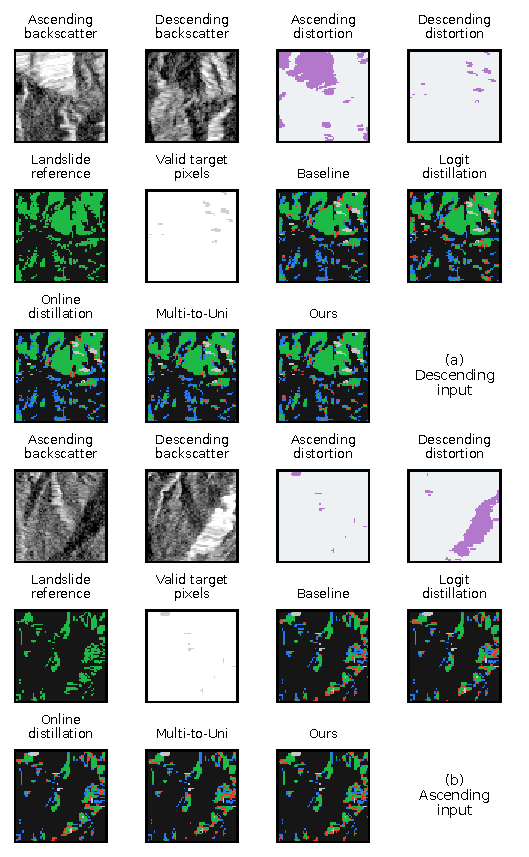
\includegraphics[width=\columnwidth]{figures/fig_comparison_valid_reader.pdf}
\caption{Valid-pixel comparison for descending-input and ascending-input examples. Rows show both post-event radar views, distortion regions (purple), the landslide reference, evaluation support, and five methods. Distorted input pixels are excluded identically for every prediction (gray). Correct landslides are green; false alarms are red; missed landslides are blue.}
\label{fig:qualitative}
\end{figure}
\begin{figure}[!t]
\centering
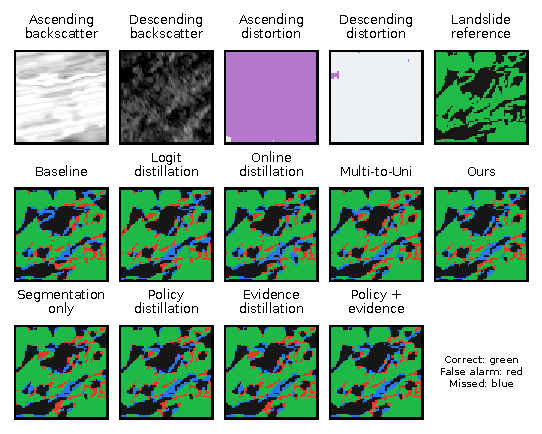
\includegraphics[width=\columnwidth]{figures/fig_comparison_full_reader.pdf}
\caption{Full-pixel comparison on an ascending-input slope. Top: both radar views, their distortion regions, and reference. Middle: five competing methods. Bottom: segmentation, policy, evidence, and both objectives under matched training. No distorted prediction is hidden. Colors follow Fig.~\ref{fig:qualitative}.}
\label{fig:full_comparison}
\end{figure}

\subsection{Complementary Guidance and Search}
Table~\ref{tab:search_intervention} separates Teacher guidance from Student sampling. The self-guided Teacher is independently trained; counter shuffling mismatches paired locations at inference. Fixed-center and random-offset tests retain learned aggregation weights; removing search feeds the fine-scale feature directly to the trained decoder. Correct pairing is beneficial, and arbitrary offsets reduce performance. Fixed-center Student sampling remains competitive, so these inference tests do not establish that learned spatial displacement is necessary.
\begin{table}[!t]
\caption{Guidance and sampling comparison (\%). Teacher rows compare guidance; Student rows alter sampling during inference.}
\label{tab:search_intervention}
\centering\scriptsize
\setlength{\tabcolsep}{2.5pt}
\begin{tabular}{lrrrr}
\toprule
Method & \multicolumn{2}{c}{Valid pixels} & \multicolumn{2}{c}{All pixels}\\
 & AUPRC & IoU & AUPRC & IoU\\
\midrule
\multicolumn{5}{l}{\emph{Teacher guidance}}\\
Self-guided & 87.74 & 62.72 & 88.15 & 63.21\\
Counter-guided & 89.04 & 65.01 & 89.48 & 65.65\\
Shuffled counter & 81.73 & 51.45 & 82.54 & 52.08\\
\midrule
\multicolumn{5}{l}{\emph{Student sampling}}\\
Learned sampling & 88.77 & 64.65 & 89.16 & 65.10\\
Fixed center & 88.71 & 64.63 & 89.10 & 65.06\\
Random offsets & 86.96 & 58.72 & 87.43 & 59.27\\
Without search & 87.90 & 64.31 & 88.31 & 64.79\\
\bottomrule
\end{tabular}
\end{table}

Fig.~\ref{fig:search_samples} shows the actual sampling and weight allocation across three feature scales. Learned points overlap, supporting an interpretation involving scale and weight allocation rather than diverse spatial displacements. Across valid query regions, Student-to-Teacher candidate-weight Jensen--Shannon divergence is 0.0219 versus 0.0782 with shuffled guidance; shared-memory cosine distance is 0.0066 versus 0.0595. Candidate-weight divergence summarizes the twelve weights; training instead aligns the spatial sampling distributions.
\begin{figure}[!t]
\centering
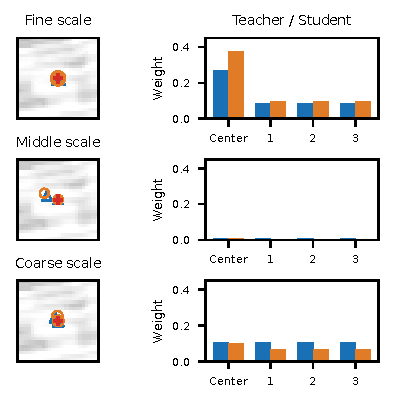
\includegraphics[width=\columnwidth]{figures/fig_search_reader.pdf}
\caption{Teacher (blue triangles) and Student (orange circles) sampling at fine, middle, and coarse scales. The red cross marks the query; bars show candidate weights. Overlapping learned samples are displayed at their actual locations. Each scale has one fixed center and three coincident learned candidates.}
\label{fig:search_samples}
\end{figure}

\subsection{Distillation Objectives}
Table~\ref{tab:loss_parts} compares matched segmentation, policy, evidence, and combined objectives. Policy distillation improves the segmentation control, whereas evidence alone gives essentially unchanged accuracy. The combined Student obtains the highest AUPRC and IoU in both reported domains. The matched segmentation control is stronger than the primary baseline because it is separately retrained under the current schedule; the two controls are not interchangeable. These single-run comparisons do not establish statistical superiority.
\begin{table}[!t]
\caption{Distillation objectives under matched training (\%). The surviving objective retains its original coefficient.}
\label{tab:loss_parts}
\centering\scriptsize
\setlength{\tabcolsep}{2.5pt}
\begin{tabular}{lrrrr}
\toprule
Method & \multicolumn{2}{c}{Valid pixels} & \multicolumn{2}{c}{All pixels}\\
 & AUPRC & IoU & AUPRC & IoU\\
\midrule
Segmentation only & 88.28 & 63.48 & 88.69 & 64.07\\
Policy distillation & 88.55 & 63.88 & 88.96 & 64.45\\
Evidence distillation & 88.28 & 63.45 & 88.68 & 64.02\\
Policy + evidence & 88.77 & 64.65 & 89.16 & 65.10\\
\bottomrule
\end{tabular}
\end{table}

